\chapter{Redes de Petri}
\label{chap:petri}

\section{Modelagem de Sistemas}
Para a modelagem de sistemas é importante entender as principais características do sistema que está sendo estudado, no propósito de uma revisão na classificação de sistemas,foi elencado em \cite{cassandras} tais classificações, observe que elas não são necessariamente auto exclusivas: 

\textbf{Sistema Dinâmico e Estático:}  Em sistema estático a saída é sempre independente dos valores de entrada passados, já em um sistema dinâmico os valores de saída dependem dos valores anteriores da entrada. Equações diferencias ou a diferença são geralmente requeridas para representar o comportamento de sistemas dinâmicos.

\textbf{Sistema Variante e Invariante no Tempo:} Em um sistema invariante no tempo o comportamento do mesmo não se altera com o passar do tempo. Tal sistema é dado com estacionário pois se aplicada a mesma entrada ao longo do tempo o sistema responderá com o mesmo comportamento.

\textbf{Sistemas Lineares e Não Lineares: } Um sistema linear obedece a condição $g(a_1u_1 + a_2u_2) = a_1g(u_1) + a_2g(u_2)$ tais que $u_1$ e $u_2$ são dois vetores de entrada, $a_1$ e $a_2$ dois números reais e $g(.)$ é a saída resultante. 

\textbf{Sistema em Estado Contínuo e Discreto: } Um sistema contínuo pode ter a variável de estado representa por um número real ou complexo, já o sistema discreto é representado por uma série de elementos discretos.

\textbf{Sistema Orientado a Eventos e Tempo: } Em um sistema orientado ao tempo o estado do sistema muda com a mudança de tempo, já a eventos a mudança de estado ocorre de forma instantânea a partir da ocorrência de um evento.

\textbf{Sistema Determinístico e Estocástico: } Um sistema se torna estocástico quando possui uma ou mais de uma variável estocástica. Nesse caso o estado do sistema é descrito por um processo estocástico.

\textbf{Sistema em Tempo Contínuo e Discreto: } Um sistema em tempo contínuo possui todas as entradas definidas para todos os valores de tempo possíveis. 

No escopo do trabalho proposto o a modelagem em redes de petri é utilizada para um sistema a eventos discretos seguindo a seguinte árvore de escopos dada pela figura \ref{fig:arvore_escopo}
\begin{figure}
    \centering
    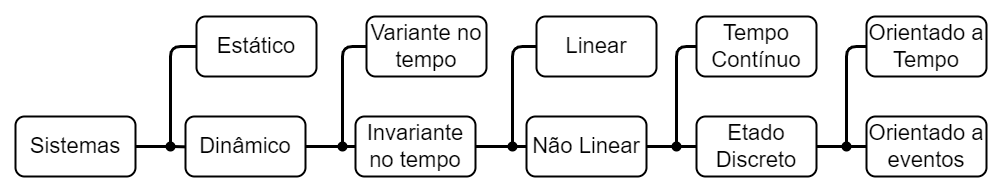
\includegraphics[scale=0.4]{figures/Petri/arvore_escopo.png}
    \caption{Árvore de escopo de um sistema a eventos discretos }
    \label{fig:arvore_escopo}
\end{figure}

  % \centering
  %   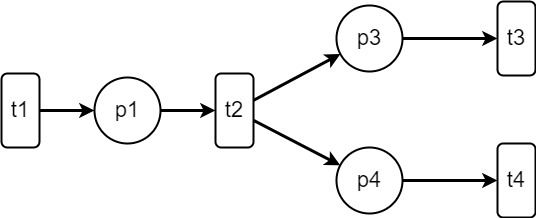
\includegraphics[scale=0.4]{figures/Petri/paralelismo_sincrono.jpg}
  %   \caption{Exemplo paralelismo Síncrono} 
  %   \label{fig:paralelismo_sincrono}
    
\subsection{Modelagem de sistemas a eventos discretos}

Em si tratando da modelagem de sistemas a eventos discretos tem-se três elementos principais utilizados na modelagem eventos(instantes e mudanças de estados), atividades(evolução do sistema físico entre dois eventos) e processos (sequência de eventos e atividades no sistema). 

Na evolução dos processos no sistema os processos podem ocorrer de forma totalmente independente entre si, enquanto outras atividades necessitam de uma determinada sincronização ou até uma sequência de eventos prévios. Uma forma de diferenciação de interações entre processos é apresentada por \cite{vallete}, como:

\textbf{Cooperação:} Os processos convergem para um objetivo comum, de modo que anteriormente há uma relativa independência antes do ponto de sincronização.

\textbf{Competição:} Os processos necessitam de um dado recurso, caso esse recurso seja abundante para todos os processos, dados processos poderiam ser descritos de forma independente, caso contrário faz-se necessário o compartilhamento de recursos envolvendo uma exclusão mútua a partir de um ponto de sincronização.

\textbf{Pseudo-Paralelismo:} O paralelismo é apenas aparente e os eventos por mais que sejam independentes nunca serão simultâneos pois são acionados por um relógio comum, a exemplo de um sistema operacional que por mais que processe várias tarefas, porém o processador só processa um ciclo de instrução por vez.

\textbf{Paralelismo Verdadeiro:} Os eventos podem ocorrer de forma simultânea, não existindo uma escala de tempo em comum, a exemplo de vários processadores operando tarefas distintas.

\section{Representação em máquina de estados}
Uma das representações mais clássicas para modelagem de sistemas à eventos discretos é a máquina de estados, para o caso de uma número de estados finitos enumera-se os possíveis estados e descreve-se os eventos referente as mudanças de estado, descrevendo-se assim cada estado a a partir do estado anterior.

O modelo matemático para a máquina de estado finita é dada a partir da equação \ref*{eq:finit_state_machine_equation}, em que $E$ é um conjunto finito de estados, dado pelo estado inicial $E_0$, um alfabeto de entrada $A$, e uma função de transição de estados $\theta$, dado por $\theta : E \times A \rightarrow E$, associando cada par de estado-entrada ao próximo estado.

\begin{equation}\label{eq:finit_state_machine_equation}
\hspace{6cm} % Adjust the value as needed
    M = (E; A; \theta; E_0)
\end{equation}
De acordo com \cite{vallete} este modelo explicita a noção de eventos e parcialmente a de atividade, não explicitando, entretanto, a noção do processo com as evoluções simultâneas de diversos processos paralelos, de modo que uma máquina de estado finita descreve apenas um único processo sequencial.

\subsection{Modelagem de processos sequenciais}
Para a descrição de vários processos sequências, uma das soluções é representar o sistema por um conjunto de máquinas de estados finitos. Quando as máquinas de estados são independentes, esse modelo se aplica sem dificuldade, porém quando existe competição ou cooperação entre os processos faz-se necessário o uso de processos sequenciais comunicantes. A sincronização é descrita através da intervenção na função de transição de estados $\theta$ de uma máquina.

\subsubsection{Representação com refinamentos sucesssivos}
Um dos contrapontos dessa abordagem é que independente do método utilizado, a representação das comunicações entre as máquinas é diferente da representação interna da sequência de uma máquina. Portanto, tal abordagem não é compatível com a abordagem top-down de refinamento sucessivos. É necessário desde do início da modelagem a escolha de uma decomposição que não será colocada em causa a posteriori. 

\subsubsection{Explosão combinatória}
Outro ponto de análise dessa forma de modelagem é que para cada informação partilhada entre as máquina ou troca de sinais entre as máquinas é necessário analisar o comportamento global do sistema através do recálculo de uma nova máquina de estado que descreva o sistema de forma global. Neste caso, ocorre a problemática da explosão combinatória do número de estados definida pela relação entre $k$ máquinas e $n$ estados, produzindo uma máquina de $n^k $ estados, ocorrendo uma explosão combinatória a medida que k e n aumentam.

\subsubsection{Não-independência de submáquinas e bloqueio}
Em se tratando de sistemas com paralelismo um dos problemas comuns que podem acontecer é o de bloqueio (dead-lock) em que a máquina de estado não consegue evoluir pois depende da transição de um estado de outra máquina que por sua vez encontra-se igualmente no mesmo estado de espera. Existem técnicas na teoria de máquinas de estados finitos que evitam o bloqueio, porém a estrutura do sistema acaba sendo comprometida, perdendo assim a representativa clara do sistema e suas transições.

\section{Modelagem utilizando Rede de Petri}

A rede de Petri é uma ferramenta gráfica e matemática para modelagem e controle de sistemas à eventos discretos, dado que o sistema a ser escolhido é um sistema que pode ser modelado através de tal ferramenta, com o intuito de obter uma visualização gráfica do processo, implementar lógica de controle e sincronismo, analisar propriedades da rede entre outras.

A descrição dos eventos e transições do sistema é dada através da rede de petri pelos lugares, fichas e transições, para representar os "estados" do sistema são utilizados os lugares, já as transições movimentam os recursos, ou seja, as fichas de um lugar para outro, dada a condição que a transição só possa ser disparada caso os lugares a ela ligada estejam completas com os recursos requisitados, fazendo assim interdependências em que um determinado estado só pode ser alcançado caso determinadas condições satisfeitas.

O comportamento dinâmico do sistema se dá através do disparo das transições, evento que faz com que o sistema passe do estado atual para o próximo estado. Tal disparo consiste em duas etapas, a primeira de retirar as fichas dos lugares de entrada e por fim depositar as fichas em cada lugar de saída.

\subsection{Evolução síncrona e assíncrona}
A rede de petri pode representar sistemas com eventos síncronos e assíncronos, em que são necessários momento de espera para acontecer determinados eventos assim como a independência de eventos que podem ou não ocorrer de forma simultânea.

Observa-se na figura \ref{fig:paralelismo_sincrono} um evento caracterizado como divisão em que no disparo da transição $t_2$ uma ficha é retirada de $p_1$ e simultaneamente é colocada uma ficha em $p_3$ e $p_4$ daí em diante a evolução do sistema ocorre de forma assíncrona podendo ou não haver disparos concorrentes.  

\begin{figure}[h]
    \centering
    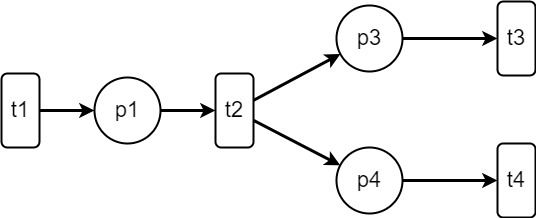
\includegraphics[scale=0.4]{figures/Petri/paralelismo_sincrono.jpg}
    \caption{Exemplo paralelismo Síncrono} 
    \label{fig:paralelismo_sincrono}
\end{figure}

Observa-se na figura \ref{fig:paralelismo_assincrono} um evento caracterizado como junção em que para haver o disparo de $t_3$ é necessário que haja uma ficha tanto em $p_3$ quanto em $p_4$, o consumo dessas fichas ocorre de forma síncrona tal evento implica necessariamente de uma espera em que ou $p_3$ espera a chegada do recurso em $p_4$ ou o contrário, garantindo assim que $p_5$ só receba uma fica quando essas duas condições forem satisfeitas. Antes do disparo de $t_3$ o sistema pode evoluir de forma assíncrona com disparos independentes de $t_1$ e $t_2$.

\begin{figure}[h]
    \centering
    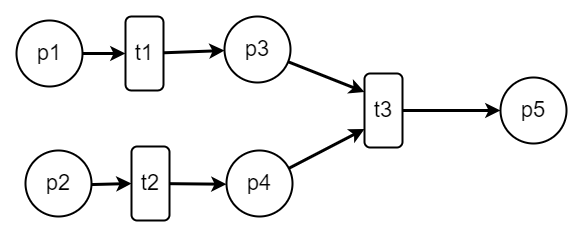
\includegraphics[scale=0.4]{figures/Petri/paralelismo_assincrono.png}
    \caption{Exemplo paralelismo Assíncrono}
    \label{fig:paralelismo_assincrono}
\end{figure}


\subsection{Caminhos alternativos e Repetição}
Um evento que também pode ser modelado são o de caminhos alternativos e variações de sequência de disparos em uma rede de petri, em que em determinado momento na rede há um lugar ligado a entrada de uma ou mais transições, ocorrendo assim a sensibilização de tais transições, podendo ocorrer portanto o disparo de qualquer uma das transições, tomando-se assim um caminho alternativo caso outra transição fosse disparada.

Observa-se esse fenômeno na modelagem descrita pela figura \ref{fig:caminhos_alternativos}, em que no momento em que $p_1$ recebe uma ficha é sensibilizada as transições $t_1$ e $t_2$, de modo que a rede de petri não restringe a escolha de um ou outra transição, porém caso uma transição seja disparada a outra não poderá ser, ocorrendo assim uma competição pelo recurso em que a transição que disparar primeiro recebe o recurso. Dado a ocorrência da repetição da rede através de $t_5$, novamente a tomada de decisão entre $t_1$ e $t_2$ ocorrera, podendo assim ocorrer um caminho alternativo ao caminho prévio dada a sequência de disparo ocorrida.

A figura \ref{fig:caminhos_alternativos}, também modela um evento de repetição através da transição $t_5$, em que dada a chegada da ficha no lugar $p_5$ tal ficha pode retornar ao lugar de origem $p_1$ ocorrendo assim o restabelecimento da rede e infinitas repetições.

\begin{figure}[ht]
    \centering
    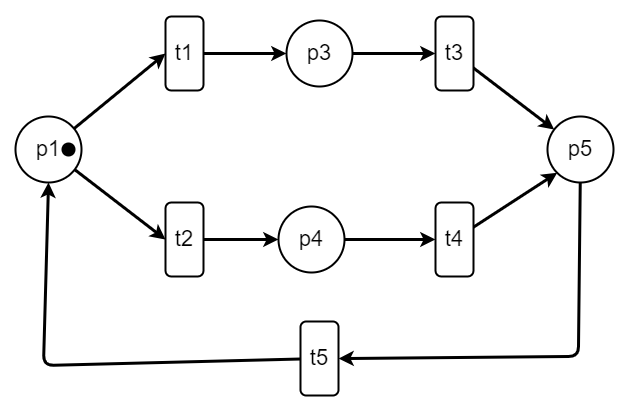
\includegraphics[scale=0.4]{figures/Petri/caminhos_alternativos.png}
    \caption{Exemplo de Caminhos alternativos e Repetição}
    \label{fig:caminhos_alternativos}
\end{figure}

\section{Redes de Petri}
A rede de Petri é uma ferramenta gráfica e matemática para modelagem e controle de sistemas à eventos discretos, dado que o sistema a ser escolhido é um sistema que pode ser modelado através de tal ferramenta, com o intuito de obter uma visualização gráfica do processo, implementar lógica de controle e sincronismo, analisar propriedades da rede entre outras.
Para a modelagem proposta utilizou-se a ferramenta do CPN Tools, assim como as funcionalidades envolvendo hierarquia para maior legibilidade da rede.

De acordo com \cite{cassandras}, os eventos na RP são relacionados as transições, de modo que para que aconteça o disparo de uma transição é necessário satisfazer determinadas condições inscritas na rede.
As informações relacionadas a tais condições estão contidas em lugares, que são vistos como "entradas" das transições. Lugares, transições e as relações entre eles são os componentes básicos de uma RP. A RP possuí dois tipos de nós, lugares e transições, e os arcos que conectam eles. Na definição de grafos a RP é classificada com um grafo bipartido de modo que os arcos não podem conectar diretamente dois nós do mesmo tipo, exemplo lugar a lugar ou transição a transição.
A definição de grafo é dada a seguir.

\subsection{Linguagem Formal}
A Rede de Petri é definida como um grafo bipartido ponderado, dado pelo conjunto $(P,T,A,w,x)$, tal que:
\begin{itemize}
    \item $P$ é o conjunto finito de lugares (um tipo de nó na grafo)
    \item $T$ é o conjunto finito de transições (o outro tipo de nó no grafo)
    \item $A \subseteq (P \times T) \cup (T \times P)$ é o conjunto de arcos dos lugares para as transições e das transições para os lugares no grafo.
    \item  $w : A \rightarrow \{1, 2, 3, \ldots\}$ são as funções de ponderação dos arcos.
    \item $x$ : é a marcação da rede de Petri dada pela função $x : P \rightarrow \mathbb{N} = \{0, 1, 2, \ldots\}$, tal marcação é definida como um vetor linha $x = x(p_1), x(p_2), ..., x(p_n)$, tal que $n$, é o número de lugares na rede.
\end{itemize}
É considerado que em $(P,T,A,w)$, não tem lugares em transições isolados.
Na representação em grafos os lugares $P = {p_1,p_2,p_3, ..}$ são representados com um círculo, as transições $T = {t_1,t_2,t_3,...}$ como retângulos.Os conjunto de arcos $A = {w_1,w_2,w_3,...}$, cada arco $w$ é representado em função de um lugar e uma transição e o peso associado como $w(p_i,t_j) = W$, tal que o arco liga o lugar $p_i$ a transição $t_j$ e possui o peso igual a $W$. A marcação no grafo é dada como fichas (ponto preto) no lugar marcado $p_i$ tal que $x(p_i) \in \mathbb{N}$.
Um exemplo de rede com os elementos citados é representado pelo grafo na figura \ref{fig:ex_rp}.

\begin{figure}[ht]
    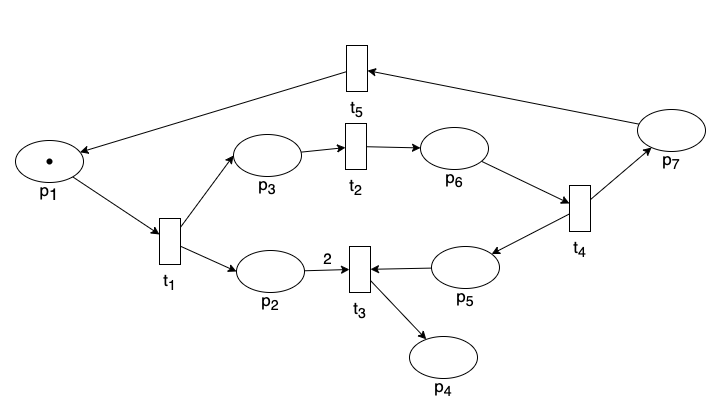
\includegraphics[scale=0.6]{figures/Petri/exemplo_rp.png}
    \caption{Exemplo de Rede de Petri}
    \label{fig:ex_rp}
\end{figure}

Tem-se x lugares, .. . ..
 ..
  . .. 
  . . .
   . . .
   
%\subsection{Redes de Petri Colorida}
%As redes de Petri  coloridas são uma ferramenta gráfica e matemática que se adaptam bem a um grande numero de aplicações, tais como protocolos de comunicação, controle de oficinas de fabricação. 

%% Apresentar em formato de quadro.